% Prezentacja artykułu bazowego (8.11): 8 slajdów, do 5 minut.
% Kompilacja: latexmk -pdf presentation.tex (obok muszą leżeć model_ranking.pdf, conditions_heatmap.pdf i examples.pdf).
% Dane sprawdzone 2.11.2026: strona wydawcy, wykaz ministerialny, Scopus.
\documentclass[aspectratio=169,11pt]{beamer}
\usepackage[T1]{fontenc}
\usepackage[utf8]{inputenc}
\usepackage{polski}
\usepackage{lmodern}
\usepackage{booktabs}
\usepackage{array}
\usepackage{hyperref}

\usetheme{default}
\usecolortheme{seahorse}
\setbeamertemplate{navigation symbols}{}
\setbeamertemplate{footline}[frame number]
\definecolor{akcent}{rgb}{0.2,0.2,0.7}
\setbeamercolor{block title}{bg=akcent!18,fg=akcent!70!black}
\setbeamercolor{block body}{bg=akcent!6}
\setbeamerfont{block title}{size=\small,series=\bfseries}

% Wąska kolumna z etykietą po lewej, bez justowania, bo w wąskich kolumnach rozciąga odstępy.
% Bez \leavevmode kolor przesuwa pierwszy wiersz komórki o linię w dół.
\newcolumntype{L}[1]{>{\raggedright\arraybackslash\leavevmode\color{akcent!70!black}}p{#1}}
\newcolumntype{P}[1]{>{\raggedright\arraybackslash}p{#1}}
% Treść ramki o stałej wysokości, żeby sąsiednie ramki miały równą wysokość.
\newenvironment{rowna}[1]{\vspace*{-0.5\baselineskip}\begin{minipage}[t][#1][t]{\linewidth}\vspace{0pt}\raggedright}{\end{minipage}}
\newsavebox{\lewakolumna}
\newcommand{\zrodlo}[1]{\par\vfill{\tiny\color{black!65}#1\par}}

\title{Benchmarking OCR and vision-language models for Turkish text recognition: a comprehensive evaluation using synthetic data}
\subtitle{Y.~Yılmaz, E.~G.~Hanoğlu, A.~G.~Özkan, K.~Öztoprak\\
  \emph{International Journal on Document Analysis and Recognition}, Springer, 2026,
  \href{https://doi.org/10.1007/s10032-026-00613-6}{doi:10.1007/s10032-026-00613-6}}
\author{Marek Siuzdak, Maciej Pietras, Anton Ovod, Paweł Podgórski}
\date{8.11.2026}

\begin{document}

% 1 --------------------------------------------------------------------------
\begin{frame}
  \titlepage
\end{frame}

% 2 --------------------------------------------------------------------------
\begin{frame}{Czasopismo, wydawca i~autorzy}
  \sbox{\lewakolumna}{\small
    \begin{tabular}[t]{@{}L{2.15cm}P{\dimexpr0.60\textwidth-2.15cm-2\tabcolsep\relax}@{}}
      Czasopismo & \emph{International Journal on Document Analysis and Recognition} (IJDAR) \\[3pt]
      Wydawnictwo & Springer (Springer Nature) \\[3pt]
      Impact Factor & \textbf{1,7}; pięcioletni 2,3 (2025) \\[3pt]
      Punkty ministerialne & \textbf{100} (informatyka techniczna i~telekomunikacja) \\[3pt]
      Tytuł artykułu & \emph{Benchmarking OCR and vision-language models for Turkish text recognition:
        a comprehensive evaluation using synthetic data} \\[3pt]
      Typ artykułu & Original Paper (nowe badania)
    \end{tabular}}
  \begin{columns}[T]
    \begin{column}{0.60\textwidth}
      \usebox{\lewakolumna}
    \end{column}
    \begin{column}{0.37\textwidth}
      \begin{minipage}[t][\dimexpr\ht\lewakolumna+\dp\lewakolumna\relax][s]{\linewidth}
        \small
        \renewcommand{\arraystretch}{1.45}
        \begin{tabular*}{\linewidth}[t]{@{}l@{\extracolsep{\fill}}c@{}}
          \toprule
          Autor & Indeks $h$ \\
          \midrule
          Yasin Yılmaz & 0 \\
          Erol Görkem Hanoğlu & 0 \\
          Ayşe Gül Özkan & 5 \\
          Kasım Öztoprak & 9 \\
          \bottomrule
        \end{tabular*}

        \vfill
        \footnotesize\raggedright
        Afiliacja wszystkich autorów: Computer Engineering, Konya Food and Agriculture University, Turcja.
      \end{minipage}
    \end{column}
  \end{columns}
  \zrodlo{Źródła: strona czasopisma (Springer), wykaz ministerialny z 5.01.2024, Scopus; stan na 2.11.2026.}
\end{frame}

% 3 --------------------------------------------------------------------------
\begin{frame}{Cel artykułu i~pytania badawcze}
  \begin{block}{Cel}
    Ocenić, jak dokładnie klasyczne silniki OCR i~modele wizyjno-językowe (VLM) odczytują tekst turecki
    i~sprawdzić, czy wyniki z~danych syntetycznych przenoszą się na prawdziwe zdjęcia.
  \end{block}
  \small
  Autorzy szukają odpowiedzi na cztery pytania:
  \begin{enumerate}
    \item Czy litery tureckie (ç, ğ, ı, İ, ö, ş, ü) zwiększają błąd odczytu?
    \item Czy długie słowa, typowe dla aglutynacyjnego tureckiego, są trudniejsze od krótkich?
    \item Czy kontekst zdania pomaga w~porównaniu z~pojedynczym słowem?
    \item Jak na błąd wpływają zniekształcenia obrazu i~typ tekstu (druk, pismo odręczne, tekst w~scenie)?
  \end{enumerate}
  \medskip
  {\normalsize \textbf{Słowa kluczowe: OCR, VLMs, Turkish text recognition, Synthetic dataset}}
\end{frame}

% 4 --------------------------------------------------------------------------
\begin{frame}{Materiał: zbiór syntetyczny i~zdjęcia}
  \begin{columns}[T]
    \begin{column}{0.48\textwidth}
      \footnotesize
      \begin{tabular*}{\linewidth}{@{}l@{\extracolsep{\fill}}r@{}}
        \textcolor{akcent!70!black}{Źródło tekstu} & Obrazy \\
        \midrule
        \emph{Nutuk} Atatürka, syntetyczne & 6600 \\
        Turecka Wikipedia, syntetyczne & 6600 \\
        \emph{Gold Standard}, zdjęcia & 90 \\
      \end{tabular*}

      \medskip
      \begin{tabular}{@{}L{1.6cm}P{\dimexpr\linewidth-1.6cm-2\tabcolsep\relax}@{}}
        Typ tekstu & Jak powstał \\
        \midrule
        Druk & 13 czcionek na tle papieru \\
        Pismo & 340 czcionek odręcznych \\
        Scena & napis wklejony w~zwykłe zdjęcia \\
        Zdjęcia & szyldy, skany, notatki (6 $\times$ 15) \\
      \end{tabular}
    \end{column}
    \begin{column}{0.48\textwidth}
      \footnotesize
      \begin{tabular}{@{}L{2.3cm}P{\dimexpr\linewidth-2.3cm-2\tabcolsep\relax}@{}}
        Kategoria & Podkategorie \\
        \midrule
        Litery tureckie & z~nimi, bez nich \\
        Długość słowa & poniżej 10, ponad 10 znaków \\
        Kontekst & pojedyncze słowo, zdanie \\
        Zniekształcenia & czysty, obrót, szum, rozmycie, niska rozdzielczość \\
      \end{tabular}

      \medskip
      \begin{tabular}{@{}L{1.6cm}P{\dimexpr\linewidth-1.6cm-2\tabcolsep\relax}@{}}
        \multicolumn{2}{@{}>{\color{akcent!70!black}}l@{}}{Generowanie obrazów} \\
        \midrule
        Obrazy & 3 typy $\times$ 11 podkategorii $\times$ 200 \\
        Narzędzie & generator TRDG~1.8.0 \\
      \end{tabular}
    \end{column}
  \end{columns}

  \vspace{6pt}
  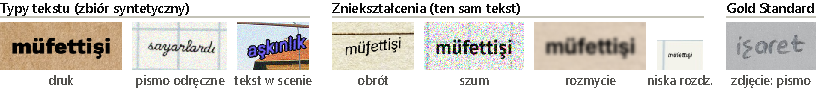
\includegraphics[width=\textwidth]{examples.pdf}\par
  \zrodlo{Przykłady: zbiór autorów na Zenodo, DOI 10.5281/zenodo.21923181 (CC~BY~4.0).}
\end{frame}

% 5 --------------------------------------------------------------------------
\begin{frame}{Metody: modele i~miary błędu}
  \begin{columns}[t]
    \begin{column}{0.46\textwidth}
      \begin{block}{10 modeli, bez douczania\vphantom{y}}
        \begin{rowna}{5.25cm}
        \footnotesize
        \begin{tabular}[t]{@{}L{1.75cm}P{\dimexpr\linewidth-1.75cm-2\tabcolsep\relax}@{}}
          OCR & PaddleOCR, TrOCR, GOT-OCR~2.0 \\[2pt]
          Otwarte VLM & Qwen2.5-VL~7B, InternVL3~8B, DeepSeek-VL2~Tiny, Phi-3.5-Vision, Pixtral~12B \\[2pt]
          Komercyjne VLM & GPT-4o, Claude Sonnet 4
        \end{tabular}

        \medskip
        Google Colab, GPU Nvidia A100; każdy model odczytuje 13\,200 obrazów syntetycznych i~90 prawdziwych zdjęć.

        \medskip
        \textbf{Polecenie dla VLM:} \emph{,,Extract the Turkish text from the image exactly as it appears\ldots''}
        \end{rowna}
      \end{block}
    \end{column}
    \begin{column}{0.51\textwidth}
      \begin{block}{Miary błędu i~analiza}
        \begin{rowna}{5.25cm}
        \footnotesize
        \textbf{CER} (błąd znakowy) $=\dfrac{S+D+I}{N}$\\[2pt]
        $S$, $D$, $I$: znaki podmienione, pominięte i~dopisane przez model; $N$: długość prawdziwego tekstu.
        CER\,=\,0,1 to średnio jeden zły znak na dziesięć.

        \smallskip
        \textbf{WER} (błąd wyrazowy): to samo na słowach, tylko dla zdań.

        \setlength{\leftmargini}{1.1em}
        \begin{itemize}
          \setlength{\itemsep}{0pt}
          \item Wielkość liter pomijana; CER powyżej 1 (gdy model dopisze wiele znaków) liczony jako 1.
          \item Przedziały ufności 95\%: metoda bootstrap.
          \item Zgodność rankingów modeli na zdjęciach i~syntetykach: korelacja Spearmana.
          \item Litery tureckie: odsetek odczytanych poprawnie.
        \end{itemize}
        \end{rowna}
      \end{block}
    \end{column}
  \end{columns}
\end{frame}

% 6 --------------------------------------------------------------------------
\begin{frame}{Wyniki: ranking modeli i~walidacja na zdjęciach}
  \begin{columns}[T]
    \begin{column}{0.62\textwidth}
      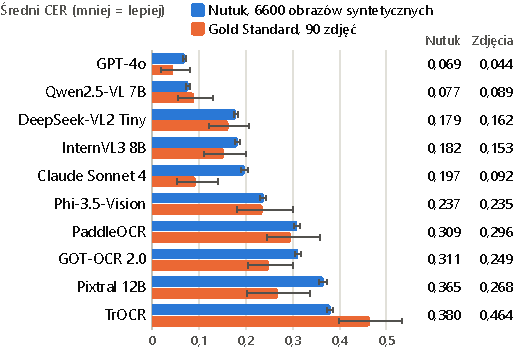
\includegraphics[width=\textwidth,height=0.80\textheight]{model_ranking.pdf}
    \end{column}
    \begin{column}{0.36\textwidth}
      \small
      \begin{itemize}
        \item GPT-4o i~otwarty Qwen2.5-VL wyraźnie przed resztą.
        \item Claude Sonnet 4: 5.~na syntetykach, 3.~na zdjęciach.
        \item TrOCR ostatni na obu zbiorach.
        \item Ranking na zdjęciach prawie taki sam jak na danych syntetycznych (Spearman $\rho=0{,}92$, $p<0{,}001$).
        \item Wikipedia: CER średnio o~3\% wyższy, kolejność prawie bez zmian.
      \end{itemize}
    \end{column}
  \end{columns}
  \zrodlo{Kreski: 95\% przedziały ufności (bootstrap).}
\end{frame}

% 7 --------------------------------------------------------------------------
\begin{frame}{Wyniki: czynniki utrudniające odczyt}
  % Klamra zaraz po tytule ramki zostałaby podtytułem, dlatego \centerline.
  \centerline{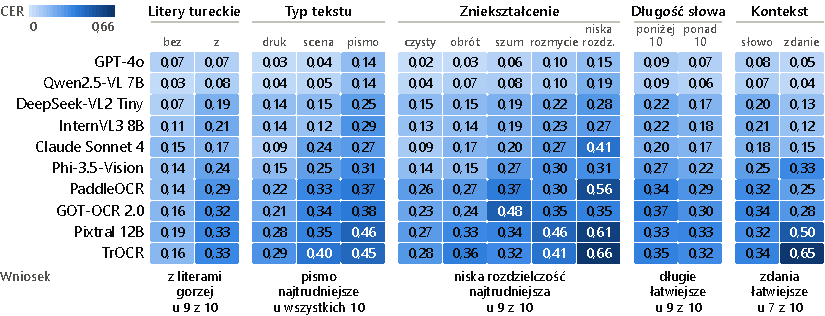
\includegraphics[width=\textwidth]{conditions_heatmap.pdf}}
\end{frame}

% 8 --------------------------------------------------------------------------
\begin{frame}{Wkład autorów i~elementy nowości}
  \begin{columns}[t]
    \begin{column}{0.48\textwidth}
      \begin{block}{Wkład autorów\vphantom{y}}
        \begin{rowna}{3.3cm}
        \small
        \setlength{\leftmargini}{1.2em}
        \begin{itemize}
          \setlength{\itemsep}{1pt}
          \item Publiczny zbiór: 13\,200 obrazów syntetycznych (druk, pismo, scena) i~90 prawdziwych zdjęć.
          \item Ocena 10 modeli z~trzech grup (klasyczny OCR, otwarte i~komercyjne VLM) na tych samych obrazach.
        \end{itemize}
        \end{rowna}
      \end{block}
    \end{column}
    \begin{column}{0.48\textwidth}
      \begin{block}{Elementy nowości}
        \begin{rowna}{3.3cm}
        \small
        \setlength{\leftmargini}{1.2em}
        \begin{itemize}
          \setlength{\itemsep}{1pt}
          \item Pierwsze porównanie OCR i~VLM dla tureckiego (wcześniej tylko klasyczny OCR).
          \item Wpływ każdego czynnika osobno: te same teksty z~różnymi zniekształceniami.
          \item Błędy dla każdej z~7 liter tureckich.
          \item Walidacja na zdjęciach: $\rho=0{,}92$.
        \end{itemize}
        \end{rowna}
      \end{block}
    \end{column}
  \end{columns}
  \vspace{8pt}
  \small
  \begin{tabular}{@{}L{3.0cm}P{\dimexpr\textwidth-3.0cm-2\tabcolsep\relax}@{}}
    Ograniczenia & pismo odręczne z~czcionek zamiast prawdziwego, modele bez dostrajania, tylko 90 prawdziwych zdjęć. \\[2pt]
    Dostęp do danych & zbiór na Zenodo (CC~BY~4.0), kod na GitHubie. \\[2pt]
    Nasze odtworzenie & 8 otwartych modeli uruchomionych ponownie: średni CER zgodny z~autorami co do 0,001 (poza Pixtralem), ranking modeli taki sam.
  \end{tabular}
\end{frame}

\end{document}
